\documentclass[a4paper]{report}
\usepackage{amsmath,mathrsfs}
\usepackage{mathtools}
\usepackage{tabularx,booktabs}
\usepackage{graphicx}
\usepackage{subcaption}
\usepackage{mdframed}
\usepackage{algorithm}
\usepackage{algorithmicx}
\usepackage{algpseudocode}
\usepackage[a4paper,margin=2.7cm,tmargin=2.5cm,bmargin=2.5cm]{geometry} 
\addtocounter{chapter}{1}
\makeatletter
\renewcommand{\thesection}{\@arabic\c@section}
\renewcommand{\thefigure}{\@arabic\c@figure}
\makeatother

\newcommand{\nexercise}[0]{\arabic{exercises}\addtocounter{exercises}{1}}

\begin{document}

%\title{\vspace{-2.0cm}SLM tutorial}
%\author{Petr Znamenskiy}

%\maketitle

\newcounter{exercises}
\addtocounter{exercises}{1}
\newmdenv[linewidth=2pt,
frametitlerule=true,
roundcorner=10pt,
linecolor=red,
leftline=false,
rightline=false,
skipbelow=12pt,
skipabove=12pt,
nobreak=true,
innerbottommargin=7pt,
]{exercisebox}

	

\section{Introduction}
Applications of Spatial Light Modulators (SLMs):
\begin{itemize}
	\item patterned illumination;
	\item wavefront shaping, adaptive optics;
	\item beam shaping.
\end{itemize}

There are other devices that can be used for patterned illumination, e.g. DMDs (Figure \ref{fig:dmd}). Some of their applications will be covered later in during the summer school. From the diagram in Figure \ref{fig:dmd}, can you guess what is the main limitation of DMDs?

\begin{figure}[b]
  \centering
  \begin{subfigure}[b]{0.4\textwidth}
      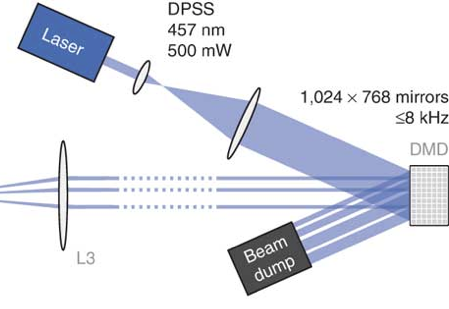
\includegraphics[width=1\textwidth]{dmd.png}
  \caption{Digital micromirror device (DMD) setup.}
  \label{fig:dmd}
  \end{subfigure}
  ~
  \begin{subfigure}[b]{0.55\textwidth}
      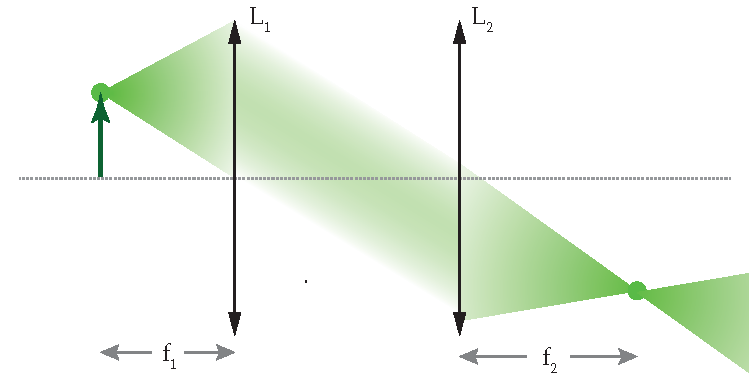
\includegraphics[width=1\textwidth]{two_lenses.pdf}
  \caption{A simple optical system.}
  \label{fig:two_lenses}  
  \end{subfigure}
  \caption{}
\end{figure}

To try to design a system for patterned illumination that gets around this limitation, lets consider a simple optical system shown in 
Figure \ref{fig:two_lenses}. How would you describe this setup? 

How is the lens $L_2$ able to create an image of the object? All $L_2$ ``sees'' is the light -- \textit{the electromagnetic field} -- created by the first lens $L_1$. If we can recreate the same electromagnetic field pattern, we generate the image without the object and $L_1$! In principle, we can create any image in the focal plane of $L_2$ (with some limitations that we will discuss later), as long as we have the tools to manipulate EM fields. 

\begin{exercisebox}[frametitle={Exercise \nexercise}: Infinite conjugate system - wavefront picture]
Draw a wavefront version of the picture in Figure \ref{fig:two_lenses} and discuss what aspects the light field between $L_1$ and $L_2$ contain the information about the position of the object.	
\end{exercisebox}

As you should appreciate, to recreate the desired image we need an ability to manipulate the phase of the light in the infinite conjugate space. \textit{Spatial light modulators} (SLMs) give us this power.

\section{SLMs as diffraction gratings}
The operating principle of SLMs is illustrated in Figure \ref{fig:slm}. LCOS-SLMs contain a \textit{liquid crystal} layer, whose orientational structure and consequently refractive index can be controlled by the electric field applied across the layer. Increasing the refractive index at a given pixel slows down the light and introduces a phase shift with respect to the rest of the wavefront.

Liquid crystals exhibit \textit{birefrigence} -- their refractive index depends on the polarization of the light. Therefore, we must ensure that that the incident beam is correctly polarized.

\begin{figure}
	\centering
    \begin{subfigure}[b]{0.69\textwidth}	
	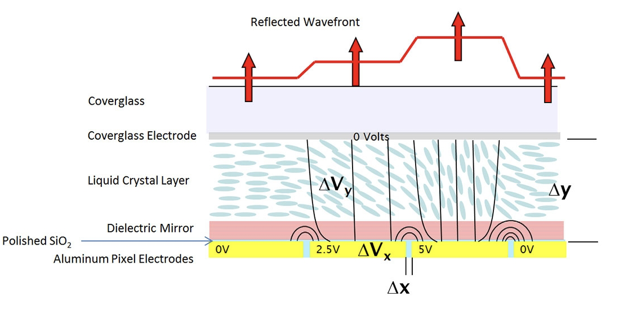
\includegraphics[width=\textwidth]{slm}
	\caption{Operating principle of an LCOS-SLM.}
	\label{fig:slm}
	\end{subfigure}
	\begin{subfigure}[b]{0.3\textwidth}	
		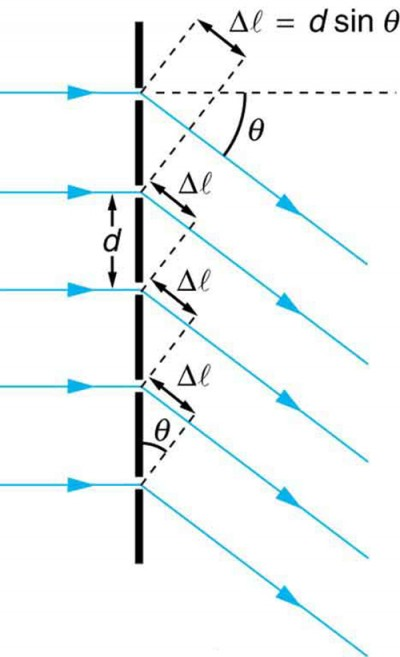
\includegraphics[width=3cm]{grating.jpg}
	\caption{Diffraction at a grating.}
	\label{fig:grating}	
	\end{subfigure}
	\caption{}
\end{figure}

\begin{exercisebox}[frametitle={Exercise \nexercise}: Grating recap]
Let's briefly recap the effects of a diffraction grating (Figure \ref{fig:grating}). At what angles $\theta$ will we observe constructive interference?
\end{exercisebox}

You can think of SLMs as programmable diffraction gratings. Rather than having slits, we can directly change the phase of the wavefront. Calibration for the SLM measures the voltage or inputs signal needs to produce a desired phase shift at a given wavelength.

\begin{exercisebox}[frametitle={Exercise \nexercise}: SLM optical setup]
Examine the optical setup on the table. Do you recognize any of the optical elements?

Next, we will power up the laser and observe the resulting diffraction pattern. What is the explanation for the pattern we observe?
\end{exercisebox}

\begin{exercisebox}[frametitle={Exercise \nexercise}: Gratings]
Next, we will load a simple grating pattern onto the SLM. What phases should we use?

As you can see each diffraction mode contains an image of the SLM chip itself. To get rid of it, we will place a lens in front of the SLM. This lens is usually referred to as the \textit{Fourier lens} for reasons that will hopefully become clear.

The lens will produce a number spots in its focal plane. What determines the position of the spots?

What happens if we increase the spatial frequency (and decrease the period) of the grating?
\end{exercisebox}

As you have seen, diffraction separates light into ``beamlets'', whose angles depend on the spatial frequency of the phase mask. The Fourier lens then focuses these beamlets into spots in the \textit{Fourier plane}. Thus, there is a one-to-one relationship between spatial frequencies of the phase mask and spatial coordinates of the generated diffraction pattern.

We will next talk about how to use the relationship to create patterns with complex shapes. But first, we need to cover a bit of math.

\newpage
\section{Very brief intro to Fourier optics}
\subsection{Waves as complex numbers}
To understand how we can generate arbitrary holographic patterns, we first need to discuss how we can represent the optical field mathematically. Let's consider a monochromatic electromagnetic wave at a single point in space. As time goes on and the electric field oscillates, the amplitude of the wave will remain constant but its phase will vary (Figure \ref{fig:complex}A).

We can describe the amplitude and the phase of the wave together as a complex number $z$ (Figure \ref{fig:complex}B). As time goes on, $z$ will trace out a circle in the complex plane, whose radius given by its modulus $|z|$ defines the amplitude of the wave, while its argument $\varphi$ defines the phase. We can convert between the two representations using Euler's formula:
\begin{equation}
	z = A e^{i\varphi} = A (\cos \varphi + i \sin \varphi)
	\label{eq:euler}
\end{equation}
The formula provides an intuitive explanation for Euler's identity, $e^{i\pi} + 1 = 0$. From here on, we will use $\varphi(z)$ as shorthand for the argument (phase) of $z$.

\begin{figure}[b]
\centering
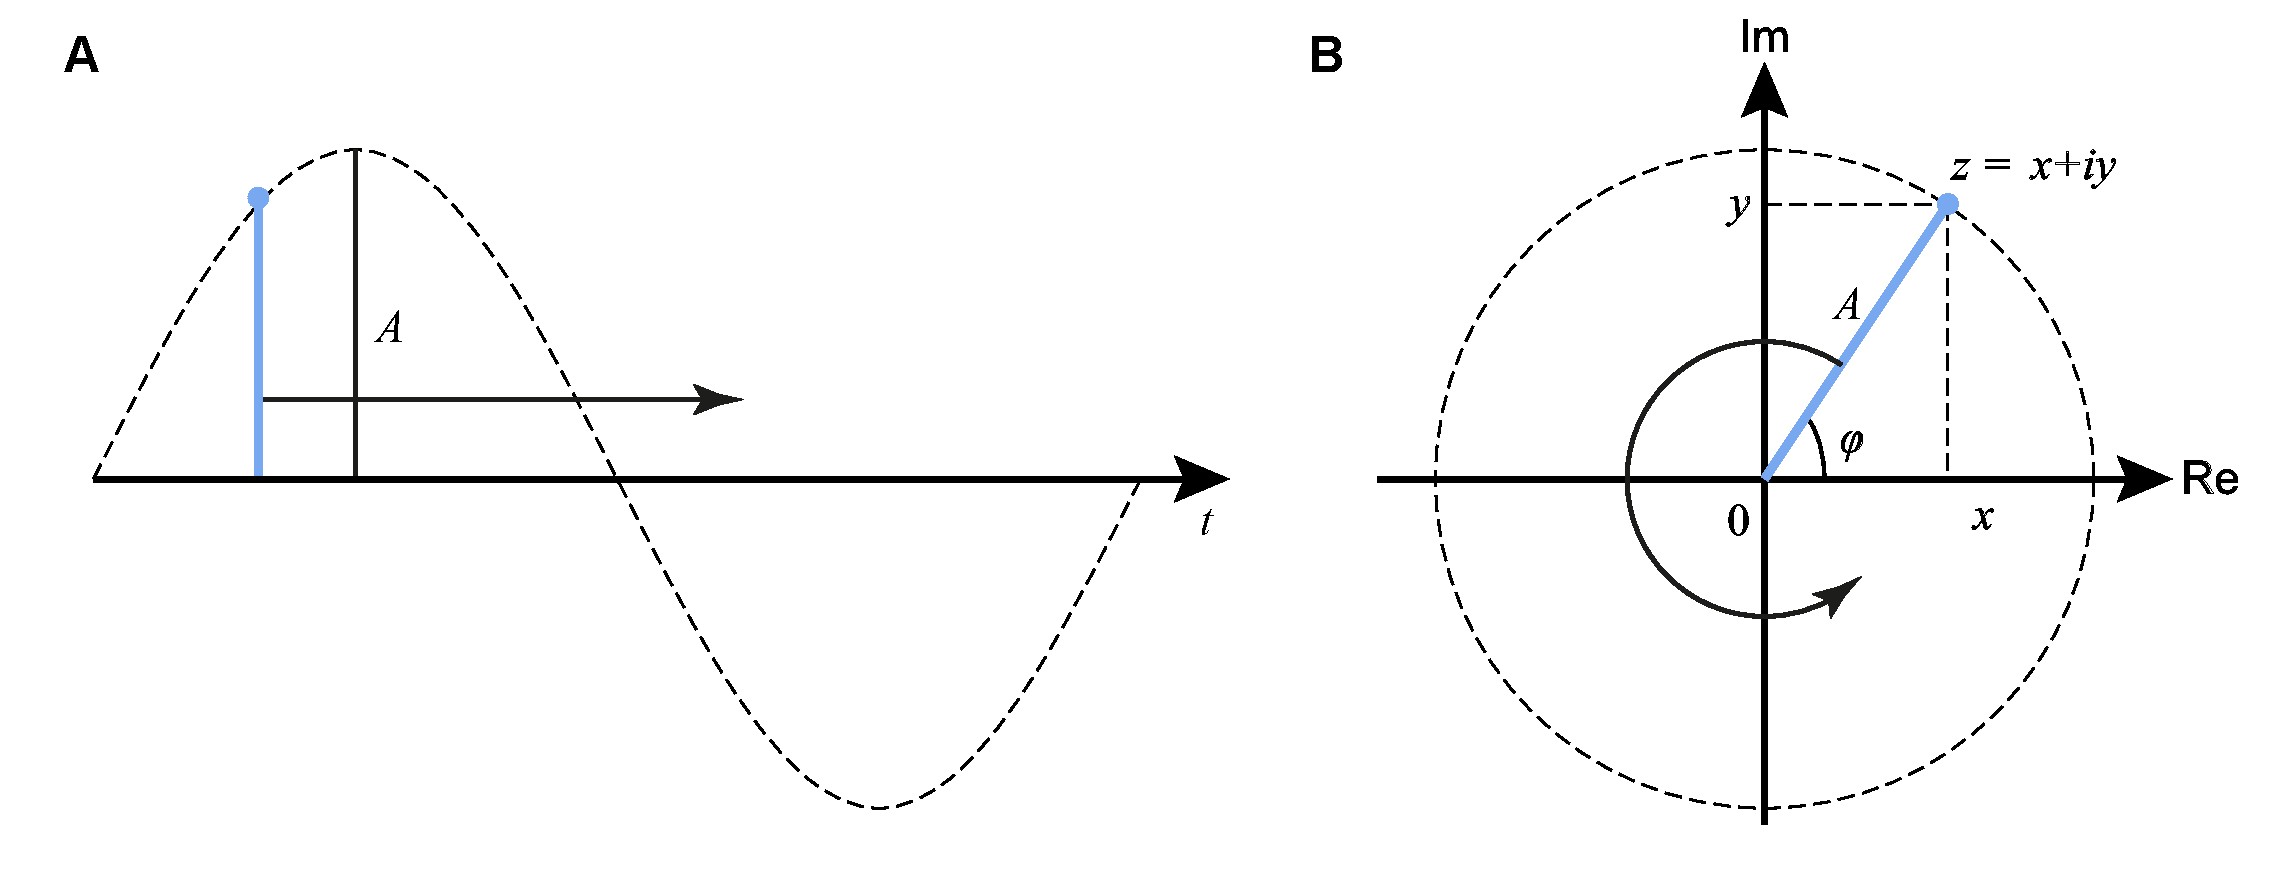
\includegraphics[width=.8\textwidth]{complex.pdf}
\caption{Representing waves as complex numbers.}
\label{fig:complex}	
\end{figure}

\subsection{The Fourier transform}
As we established above, the diffraction pattern generated by the SLM will depend on the spatial frequency content of the phase mask. Therefore, the key to creating arbitrary diffraction patterns is being able to convert between the spatial and frequency domains. This conversion is accomplished by the Fourier transform:
\begin{equation}
	\mathscr{F}[f(x)] ( u ) = \int _ { - \infty } ^ { \infty } f ( x  ) e ^ { - 2 \pi i u x } d x. 
	\label{eq:fourier}
\end{equation}
To get an intuition for it, let's focus on the second term under the integral. Following Eq. \ref{eq:euler}:

\begin{equation}
	e ^ { - 2 \pi i u x } = \cos (2 \pi u x) - i \sin (2 \pi u x),
	\label{eq:intuition}
\end{equation}
so it is a complex number, with a real part proportional to $\cos (2 \pi u x)$ and an imaginary part proportional to $- \sin (2 \pi u x)$. Therefore, if our pattern $f(x)$ lacks periodic structure at the spatial frequency $u$, if we integrate over Eq. \ref{eq:euler} the negative and positive phases of the sines and cosines will cancel out and we will end up with $\mathscr{F}[f(x)](u) = 0$. Otherwise, $\mathscr{F}[f(x)](u)$ will be a complex number~$\neq 0$, whose modulus is equal to the amplitude of the constituent component of $f(x)$ at the spatial frequency $u$.

The inverse Fourier transform is conveniently given by
\begin{equation}
	\mathscr{F}^{-1}[g(u)] ( x ) = \int _ { - \infty } ^ { \infty } g ( u ) e ^ { 2 \pi i u x } d u,
	\label{eq:invfourier}
\end{equation}
which has the same form as Eq. \ref{eq:fourier} but inverts the sign of the argument. Therefore, applying the Fourier transform twice, $\mathscr{F}[\mathscr{F}[f(x)]] = f(-x)$, we get back a spatially inverted version of the original pattern $f(x)$.

We can extend the Fourier transform to 2D:
\begin{equation}
	\mathscr{F}[f(x,y)] ( u , v ) = \int _ { - \infty } ^ { \infty } \int _ { - \infty } ^ { \infty } f ( x , y ) e ^ { - i 2 \pi ( u x + v y ) } d x d y.
\end{equation}
The intuition is the same but instead of 1D sines and cosines as in Eq. \ref{eq:intuition}, we end up with oriented 2D gratings. In the context of patterned illumination, the Fourier transform gives us the means to characterize the spatial frequency content of the phase mask, while the inverse Fourier transform allows us to select a phase mask to create a desired diffraction pattern. We will next discuss how to do this in practice.
 
\section{Creating arbitrary patterns}
From here on, $x$ and $y$ will refer to spatial coordinates in the SLM plane, while $u$ and $v$ will refer to spatial frequencies, and equivalently, to coordinates in the Fourier plane.

Suppose we would like to create a target pattern, defined by amplitudes $A_t(u,v)$ and phases $\theta_t(u,v)$. If we could use the SLM to create the optical field following the inverse Fourier transform $\mathscr{F}^{-1}[A_t(u,v) e^{i\theta_t(u,v)}]$, we would be done. However, the SLM only gives us the ability to control the phases and not the amplitudes of the light.

Fortunately, in most applications we only care about the amplitude of the target pattern $a_t(x,y)$ and not its phase. Turns out we can reproduce this amplitude pattern (with some complicated set of phases) by only manipulating the phases in the SLM plane, with the amplitudes constrained by the profile of the incident beam. To do this, we must select an SLM phase pattern $\theta_s(x,y)$ such that
\begin{equation}
\left|\mathscr{F}\left[A_s(x,y)e^{i \theta_s(x,y)}\right]\right| \approx A_t(u,v).
\end{equation}

This presents an optimization problem that can be solved iteratively using a simple algorithm summarized diagrammatically in Figure \ref{fig:gs_algorithm} and in pseudocode below. Optimiziation usually converges within just a few iterations.

\begin{exercisebox}[frametitle={Exercise \nexercise}: Generating holograms]
We will first look at the results of running Algorithm 1 with an example target pattern and convince ourselves that it indeed results in a phase pattern, whose Fourier transform has the desired amplitudes.

Next we will test this pattern on the SLM setup. Why do you think the resulting image in the Fourier plane has a ``speckled'' appearance?
\end{exercisebox}

\begin{algorithm}
\caption{Gerchberg–-Saxton algorithm} 
\label{alg1} 
\begin{algorithmic}[1]
    \Require Source amplitude pattern $A_s(x,y)$
    \Require Target amplitude pattern $A_t(u,v)$
    \Require Error tolerance $tol$
    \Ensure $|\mathscr{F}[s(x,y)]| \approx A_t(u,v)$
    \State Initialize $t(u,v) \leftarrow 0$
    \State Initialize $\epsilon \leftarrow \infty$
    \While {$\epsilon > tol$}
    	\State Reset target amplitudes but keep phases $t(u,v) \leftarrow A_t(u,v) e^{i \varphi(t(u,v))}$
    	\State Inverse FT of target pattern $s(x,y) \leftarrow \mathscr{F}^{-1}[t(u,v)]$
   		\State Reset source amplitudes but keep phases $s(x,y) \leftarrow A_s(x,y)e^{i \varphi(s(x,y))}$
   		\State Forward FT of source pattern $t(u,v) \leftarrow \mathscr{F}[s(x,y)]$
    	\State Compute error $\epsilon \leftarrow \sum_{u,v} (|t(u,v)| - A_t(u,v))^2$ 
    \EndWhile
    \State \textbf{return} $\varphi(s(x,y))$
    \end{algorithmic}
\end{algorithm}

% TODO make initilization in the diagram same as in algorithm
\begin{figure}
  \centering
      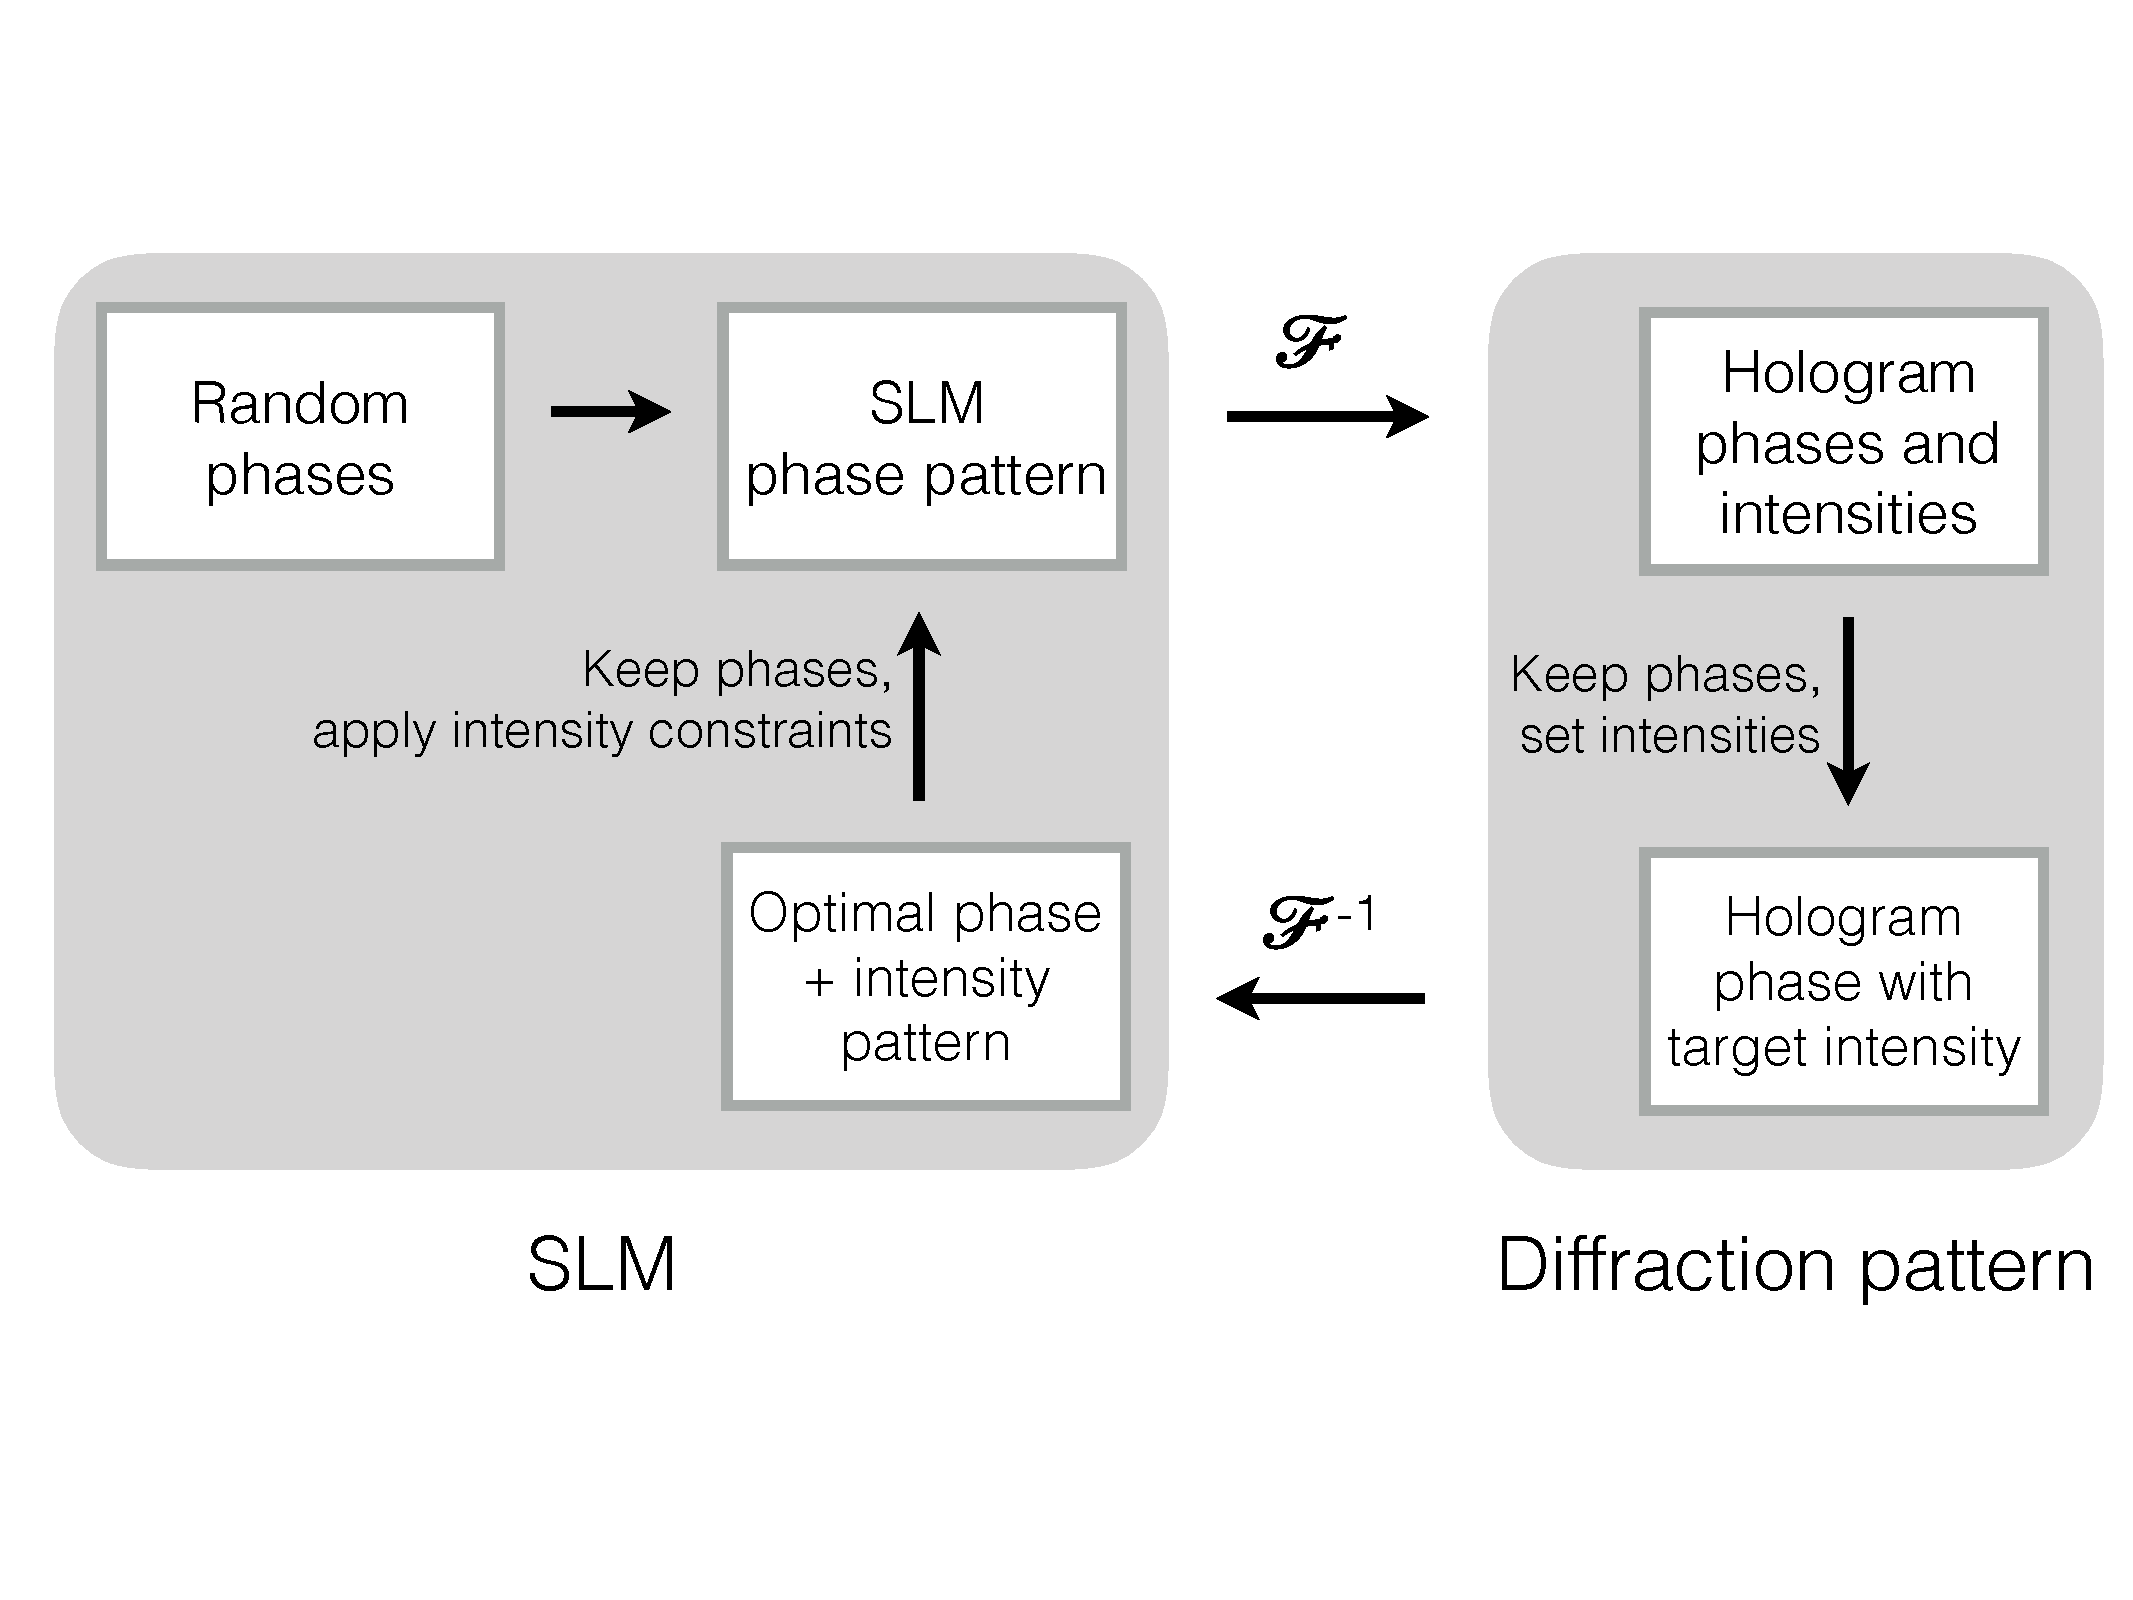
\includegraphics[width=.7\textwidth,trim={0 6cm 0 0},clip]{gs_algorithm.pdf}
  \caption{Gerchberg–-Saxton algorithm.}
  \label{fig:gs_algorithm}  
\end{figure}

\begin{exercisebox}[frametitle={Exercise \nexercise}: Practical considerations]
Think about the practical constraints of patterning light with SLMs.
\begin{itemize}
	\item What determines the resolution of the resulting pattern? 
	\item What about the field of view - the size of the largest pattern we can create?
	\item How do we integrate the SLM into a microscope to form the target pattern in the sample plane? 
\end{itemize}
\end{exercisebox}

SLMs are designed to maximize diffraction efficiency and minimize the intensity of the zero order. However, inevitably some undiffracted light will remain. We could get rid of the zero order by physically blocking it.

\begin{exercisebox}[frametitle={Exercise \nexercise}: Eliminating zero-order diffraction]
To block the zero order, we first need to make sure that our diffraction pattern is displaced from it. How can we modify the phase pattern to translate the diffraction pattern in x/y? And in z?
\end{exercisebox}

\end{document}